\section{Experiments}
In this section, we first describe our experimental setup, followed by the performance results. We then present a detailed error analysis of our dependency-based model vs. a widely-used sequential model for sentence classification. Finally, we present results for an approach that augments the textual embeddings with the user's social information.

\subsection{Experimental Setup}
We first describe our datasets, followed by comparative baselines.

\noindent
\textbf{Datasets:}
\citet{wiegand-etal-2019-detection} emphasizes the difficulty of selecting representative datasets for studying abusive language. At the heart of this difficulty is the relative rarity of hate speech in the large-scale user-generated text. It is not unusual for $> 99\%$ of text to be benign.

To make experiments manageable \citet{waseem-hovy-2016}
bootstrap data collection with queries that are indicators of possible hate speech. As a result of this bootstrapping, the data collected is {\em not} representative of the underlying text distribution. This {\em data bias} applies to both the benign and the offensive categories.

\citet{davidson2017automated} provides an alternative dataset, but this, too, is affected by pre-filtering, with the result that the dataset also fails to represent the underlying text distribution. Thus, caution is advised when interpreting the results of studies on these datasets. \citet{wiegand-etal-2019-detection} suggests several mitigations for the deficiencies of these datasets, as well as cross-classification methods that can sometimes diagnose over-optimism about classification results.

For comparability, we experiment with both the datasets from \citet{davidson2017automated} and \citet{waseem-hovy-2016}.
We do not claim that our results will necessarily transfer to more naturalistic settings. \Cref{tab:data} lists the per class distribution in the collected dataset. Note that as previously noted, \citet{davidson2017automated} dataset is highly skewed, with the majority of tweets being offensive. We thus also create a custom dataset (Davidson ext.) to mimic the real-world settings, by adding benign tweets from \citet{waseem-hovy-2016} to \citet{davidson2017automated}'s benign tweets.

\begin{table*}[h]
  \centering
  \small
\begin{tabular}{ l c c  c }
\toprule
 Dataset &  \multicolumn{3}{c}{{Categories}} \\
  \midrule
 \multirow{2}{*}{\citet{davidson2017automated}}& Hate & Offensive & Benign \\ \cline{2-4}
              & 1,430 & 19,190 & 4,163 \\
 \multirow{2}{*}{\citet{waseem-hovy-2016}}& Racism & Sexism & Benign \\ \cline{2-4}
 & 1,939 & 3,148 & 11,115 \\
 Davidson extended   &  Hate & Offensive & Benign \\ \cline{2-4}
 & 1,430 & 19,190 & 15,278 \\
 \bottomrule %\hline
\end{tabular}
\caption{\label{tab:data} Dataset Statistics. }
\end{table*}

\textbf{Baselines:}
We compare against a variety of state-of-the-art approaches proposed for computing sentence embeddings. We use these embeddings to classify the tweets into offensive or not.
\begin{itemize}
\item \textbf{N-grams} Current state-of-the-art approach for hate speech classification \cite{waseem-hovy-2016} extracts N-grams of the tweets and feed them into logistic regression along with Twitter-specific features per tweet.
%\item \textbf{Tf-Idf} approach extracts tf-idf features of each tweet which are then fed into linear SVM for classification \cite{davidson2017automated}.
\item \textbf{BERT} BERT, \citet{devlin2019bert} provides a variety of text embeddings, which have achieved new state-of-the-art results on multiple natural language tasks such as question answering and language inference. For our experiments, we initially fine-tune the $BERT_{base}$ model on our training dataset. We then extract the embeddings of each tweet from the trained model and feed them to a feedforward network to compute the final class score.

\item \textbf{BiLSTM} is a
% popular -- doesn't matter whether it is popular
sequential model to compute sentence embeddings that is useful for many downstream classification tasks \cite{bilstm}. We use the output of the final hidden layer in the BiLSTM as the sentence embeddings.
We follow BERT in feeding the sentence embeddings to a feed-forward network to compute the final class-wise score.
\end{itemize}

\noindent
\textbf{Implementation Details:}
We initialize $h_i^0$ of each word with its Glove embeddings \cite{glove} combined with its POS tag, NER tag, and dependency relation given by the Stanford NLP API. We use the Stanford parser\footnote{\url{https://nlp.stanford.edu/software/lex-parser.shtml}} for extracting the dependency parse relationship between the words in a tweet. We perform stratified sampling on the dataset to create an 80-10-10 split
between training, development and test sets. The development set is used for hyperparameter tuning while the results are reported on the test set. We report the class-wise F1 score for each dataset. We implement our model and the baselines in PyTorch and run the experiments on an Nvidia Tesla V100 GPU. We use a two-layer GCN for both DepGCN and UserGCN. We use a \emph{weighted} cross-entropy loss to counter the effect of class imbalance.
We do for all the baselines and our proposed approach.

%\noindent
\subsection{Performance Analysis:}

Table \ref{tab:davidsonext} reports class-wise F1 score with weighted F1 for the \citet{davidson2017automated} extended dataset. As expected, the bag-of-words based N-gram approach
is not competitive with the best approaches. This is reasonable, since that approach
does not take any advantage of semantic similarities between different words.
% performs the worst out of all the approaches as they do no leverage the semantic meaning of the words.
More surprisingly, the state-of-the-art BERT model, even after fine-tuning, still performs slightly worse than our DepGCN model.

\begin{table}[tbh]
  \centering
  \small
  %\setlength{\tabcolsep}{2pt}
\begin{tabular}{ l | c c  c c }
\toprule %\hline
 Approach &  Hate & Offensive & Benign & Overall \\ %\hline
  \midrule
 N-grams & 0.35 & 0.88 & 0.88 & 0.85\\
 %Tf-Idf & 0.45 & 0.94 & 0.96 \\
 BERT & 0.45 & 0.94 & 0.96 & 0.91\\
 %Emb + Pooling & 0.35 & 0.88 & 0.88 \\
 BiLSTM & 0.31 & 0.93 & 0.94 & 0.90\\
 DepGCN & 0.47 & 0.94 & 0.96 & 0.92\\
 BiLSTM + DepGCN & \textbf{0.49} & \textbf{0.95} & \textbf{0.97} & \textbf{0.93}\\
 \bottomrule %\hline
\end{tabular}
\caption{\label{tab:davidsonext} Class-wise F1 score with the overall weighted F1 score for different approaches on the \citet{davidson2017automated} extended dataset.}
\end{table}

The sequential model, i.e., BiLSTM, also performs worse than our dependency-based model. As argued before, sequential models often struggle to capture long term dependencies between words while DepGCN alleviates this issue by encoding syntactic dependencies. Further, if we use BiLSTM to contextualize the embeddings before feeding it to our DepGCN model, the results are slightly improved. Note that even a slight improvement in the hate class is significant as the dataset contains limited training examples for this class (\Cref{tab:data}) as compared to the other classes.

\begin{table}[tbh]
  \centering
  \small
  \setlength{\tabcolsep}{2pt}
\begin{tabular}{ l | c c  c c}
\toprule %\hline
 Approach &  Hate & Offensive & Benign & Overall \\ %\hline
  \midrule
 N-grams & 0.46 & 0.94 & 0.84 & 0.89 \\
 BERT & 0.42 & \textbf{0.95} & \textbf{0.88} & \textbf{0.91} \\
 %Emb + Pooling & 0.35 & 0.88 & 0.88 \\
BiLSTM & 0.52 & 0.94 & 0.86 & 0.90 \\
DepGCN & 0.50 & 0.94 & 0.86 & 0.90 \\
BiLSTM + DepGCN & \textbf{0.53} & 0.94 & 0.87 & \textbf{0.91} \\
 \bottomrule %\hline
\end{tabular}
\caption{\label{tab:davidson} Class-wise F1 score with the overall weighted F1 score for different approaches on the \citet{davidson2017automated} dataset.}
\end{table}

We obtain a similar trend in the results when evaluating performance on the original \citet{davidson2017automated} dataset, as shown in Table \ref{tab:davidson}. BERT becomes more competitive on the original dataset. The Benign class of the original dataset has systematically lower figures than the corresponding class in the extended dataset, presumably because the extended data set has a better representation of the space of possible benign examples. The Hate class is slightly easier to detect in the original dataset, even though it contains the same examples as the corresponding class in the extended dataset, presumably because the classifiers expend more of their modeling capacity on the benign set. The same pattern is present to a lesser degree for the Offensive class.
BERT becomes more competitive with BiLSTM on the original dataset. BiLSTM retains a substantial ($0.53 > 0.48$) advantage over BERT on the Hate class, and is close on Offensive and Benign.

The sequential model, BiLSTM, performs slightly better than our DepGCN model. One possible explanation can be that the \citet{davidson2017automated} dataset is full of \emph{slurs} and \emph{direct} hate attacks on entities. These \emph{direct} attacks do not exhibit long-range dependencies and thus, are well captured by the sequential models. Also, due to the heavy usage of \emph{slurs}, BERT performs worse as there are many OOV tokens in the dataset.

\begin{table}[tbh]
  \centering
  \small
  \setlength{\tabcolsep}{2pt}
\begin{tabular}{ l | c c  c c}
\toprule %\hline
 Approach &  Racist & Sexist & Benign & Overall \\ %\hline
  \midrule
 N-grams & 0.75 & 0.71 & 0.88 & 0.83 \\
 BERT & 0.78 & \textbf{0.81} & \textbf{0.91} & \textbf{0.88} \\
 %Emb + Pooling & 0.35 & 0.88 & 0.88 \\
BiLSTM & 0.72 & 0.71 & 0.89 & 0.84 \\
DepGCN & 0.76 & 0.72 & 0.88 & 0.83 \\
BiLSTM + DepGCN & \textbf{0.78} & 0.74 & 0.90 & 0.85 \\
 \bottomrule %\hline
\end{tabular}
\caption{\label{tab:waseem} Class-wise F1 score with the overall weighted F1 score for different approaches on the \citet{waseem-hovy-2016} dataset.}
\end{table}

On a more nuanced dataset collected by \citet{waseem-hovy-2016}, BERT performs the best out of the competing methods, as shown in \Cref{tab:waseem}. Our model performs competitively for racist and benign tweets while it performs worse for sexist tweets. This dataset is more nuanced as it contains more indirect or implied hate attacks (discussed in \cref{sec:error}) with the usage of fewer slurs. Thus, the powerful language model BERT can better capture the meanings of these tweets.

\begin{figure}[tbh]
\centering
\begin{subfigure}{0.45\textwidth}
%\centering
  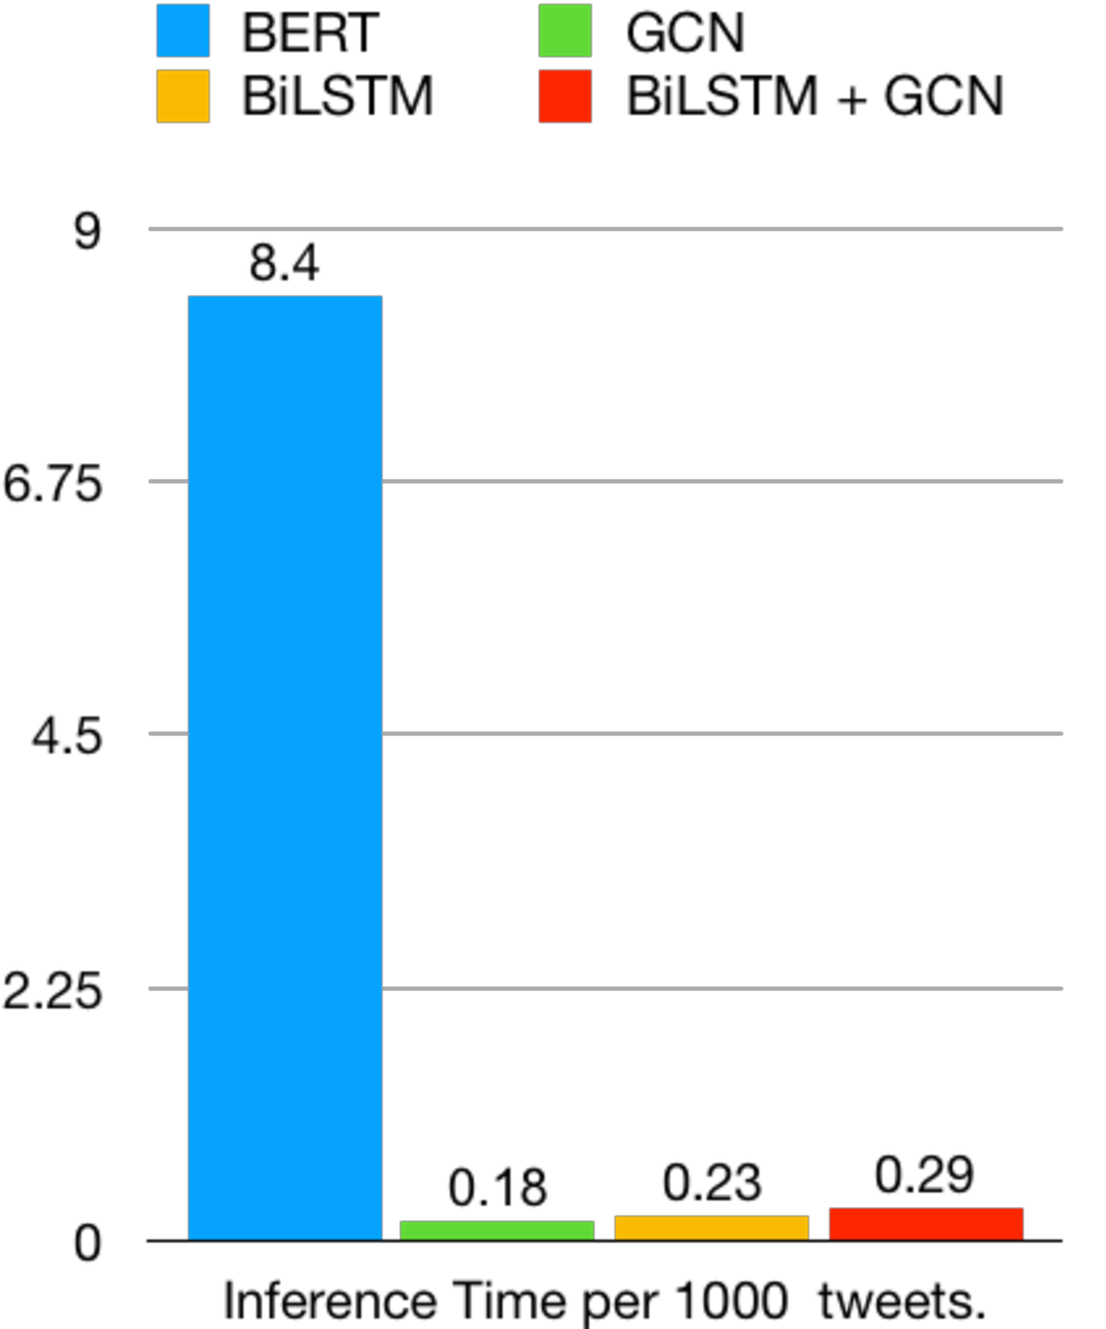
\includegraphics[scale=0.37]{figures/Traintime}
  \caption{Inference time}
  \label{fig:test}
  \end{subfigure}\hfill{}
  \begin{subfigure}{0.45\textwidth}
  %\centering
    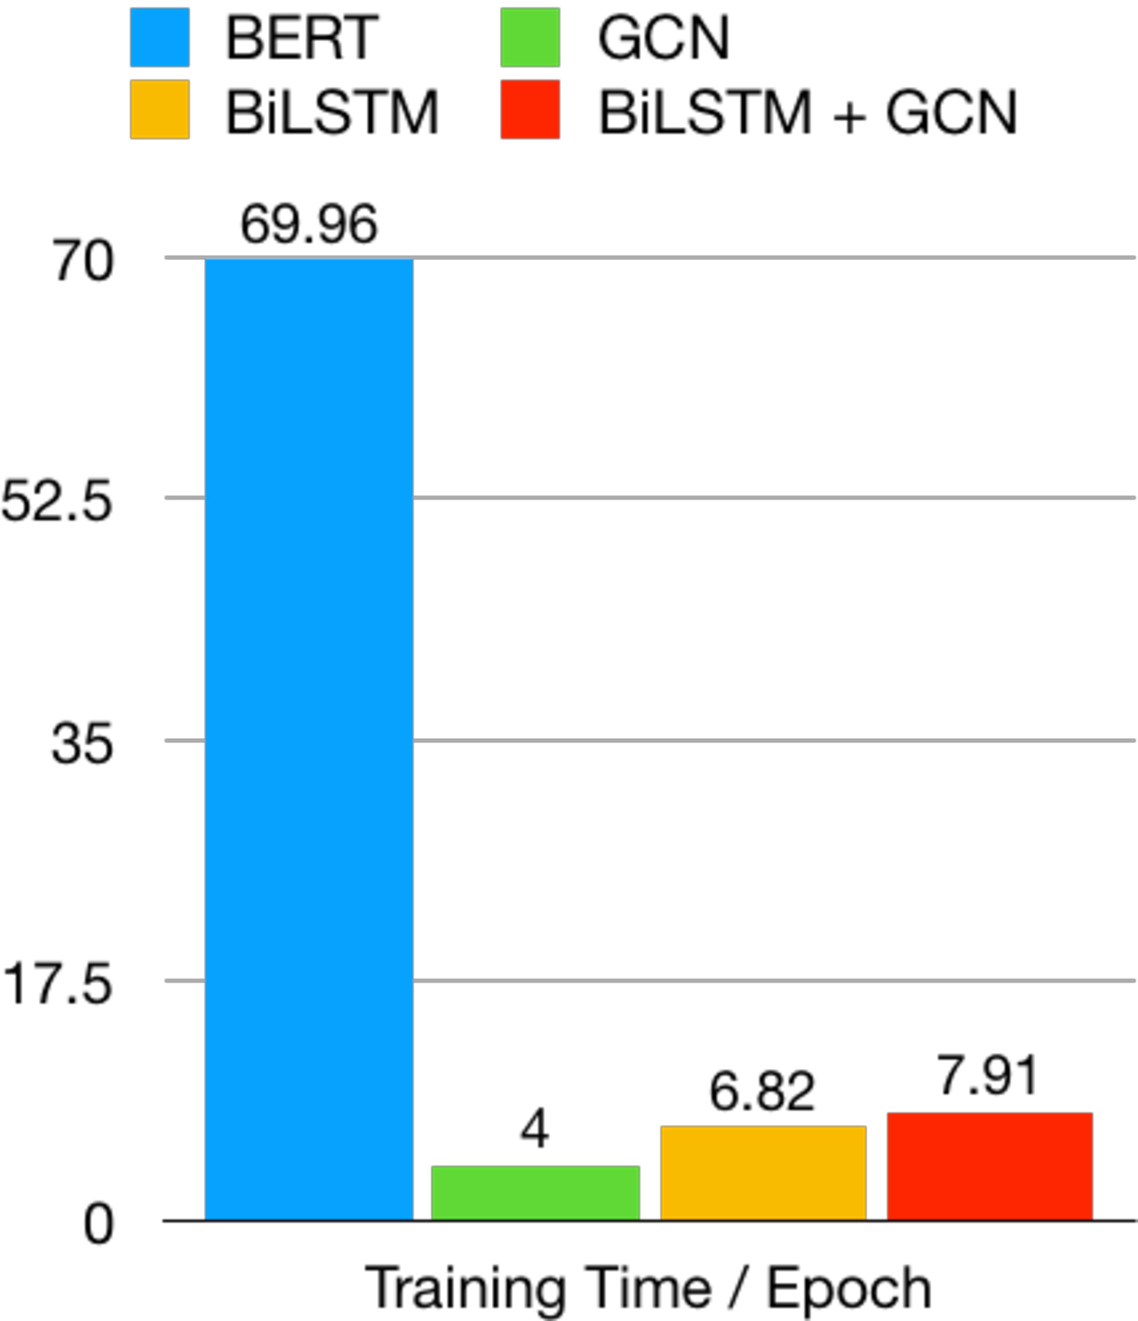
\includegraphics[scale=0.37]{figures/Testtime}
    \caption{Training time}
    \label{fig:train}
    \end{subfigure}
    \caption{\label{fig:time} Time analysis of variants of our model with respect to the popular BERT \cite{devlin2019bert} language model. }
\end{figure}

\noindent
\textbf{Time Analysis :} We further compare the running time analysis of all the baseline approaches. \Cref{fig:time} shows the comparison for both training time and inference time. First, in \Cref{fig:test}, we plot the inference time (in secs) required by each approach per 1000 tweets. Our proposed DepGCN is the most efficient approach at inference time closely followed by BiLSTM. Adding the BiLSTM module before the DepGCN only increases the inference time slightly. However, BERT, on the other hand, takes an order of magnitude longer than any of these approaches. Note that the inference time does not take into account the time taken to extract the parse tree for the tweets. However, as we are looking at a short text, this time is negligible.
The same trend can be observed for training time too in \Cref{fig:train}. However, the jump from DepGCN to BiLSTM training time is a little higher than during inference.

Thus, our parser-based DepGCN approach is much more efficient than the BERT model. Also, including BiLSTM module to the DepGCN model leads to only a slight drop in efficiency.


\subsection{Error Analysis of Sequential vs. Dependency model}
\label{sec:error}
In this section, we present a detailed analysis of the errors of the sequential (BiLSTM) vs. Dependency (DepGCN) model. Table \ref{tab:confusion} shows the confusion matrix of BiLSTM vs DepGCN model on the Waseem dataset. The parser-based approach is more conservative in labeling tweets as benign than the sequential approach. Specifically, sexist tweets are more probable to be misclassified as racist and vice versa.
Alternatively, DepGCN tags much more benign tweets as offensive (Sexist/Racist), thus creating more false positives. However, as there is a higher cost involved in missing an offensive tweet, DepGCNs will be more effective in real-world scenarios.

%\textbf{Sequential vs. Dependency based models:}

\begin{table}[tbh]
  \small
  %\setlength{\tabcolsep}{1pt}
  \begin{subtable}{0.5\linewidth}
    \centering
\begin{tabular}{ l  r  r r }
\toprule %\hline
  &  Racism & Sexism & Benign  \\ %\cmidrule(lr){2-7}
  %\hline
  \midrule
 Racism & 7 & 11 & 7 \\
 Sexism & 7 & 11 & 8 \\
 Benign & 35 & 70 & 33 \\
 \bottomrule %\hline
\end{tabular}
\caption{Dependency Parser model}
\end{subtable}%
\begin{subtable}{0.5\linewidth}
  \centering
\begin{tabular}{ l  r  r r }
\toprule %\hline
&  Racism & Sexism & Benign  \\
\midrule
Racism & 4 & 3 & 18 \\
Sexism & 1 & 7 & 18 \\
Benign & 9 & 25 & 104 \\
\bottomrule %\hline
\end{tabular}
\caption{Sequential Model}
\end{subtable}
\caption{\label{tab:confusion} Confusion matrix for Sequential (BiLSTM only) vs Dependency Parser (GCN only) approach for \citet{waseem-hovy-2016} dataset.}
\end{table}

We also examined some sample tweets from the \citet{waseem-hovy-2016} dataset, which were erroneously classified as benign by BiLSTM but not by DepGCN and vice versa to understand the difference between these two approaches in depth.

\begin{figure*}[tbh]
  \begin{subfigure}{\textwidth}
  \centering
  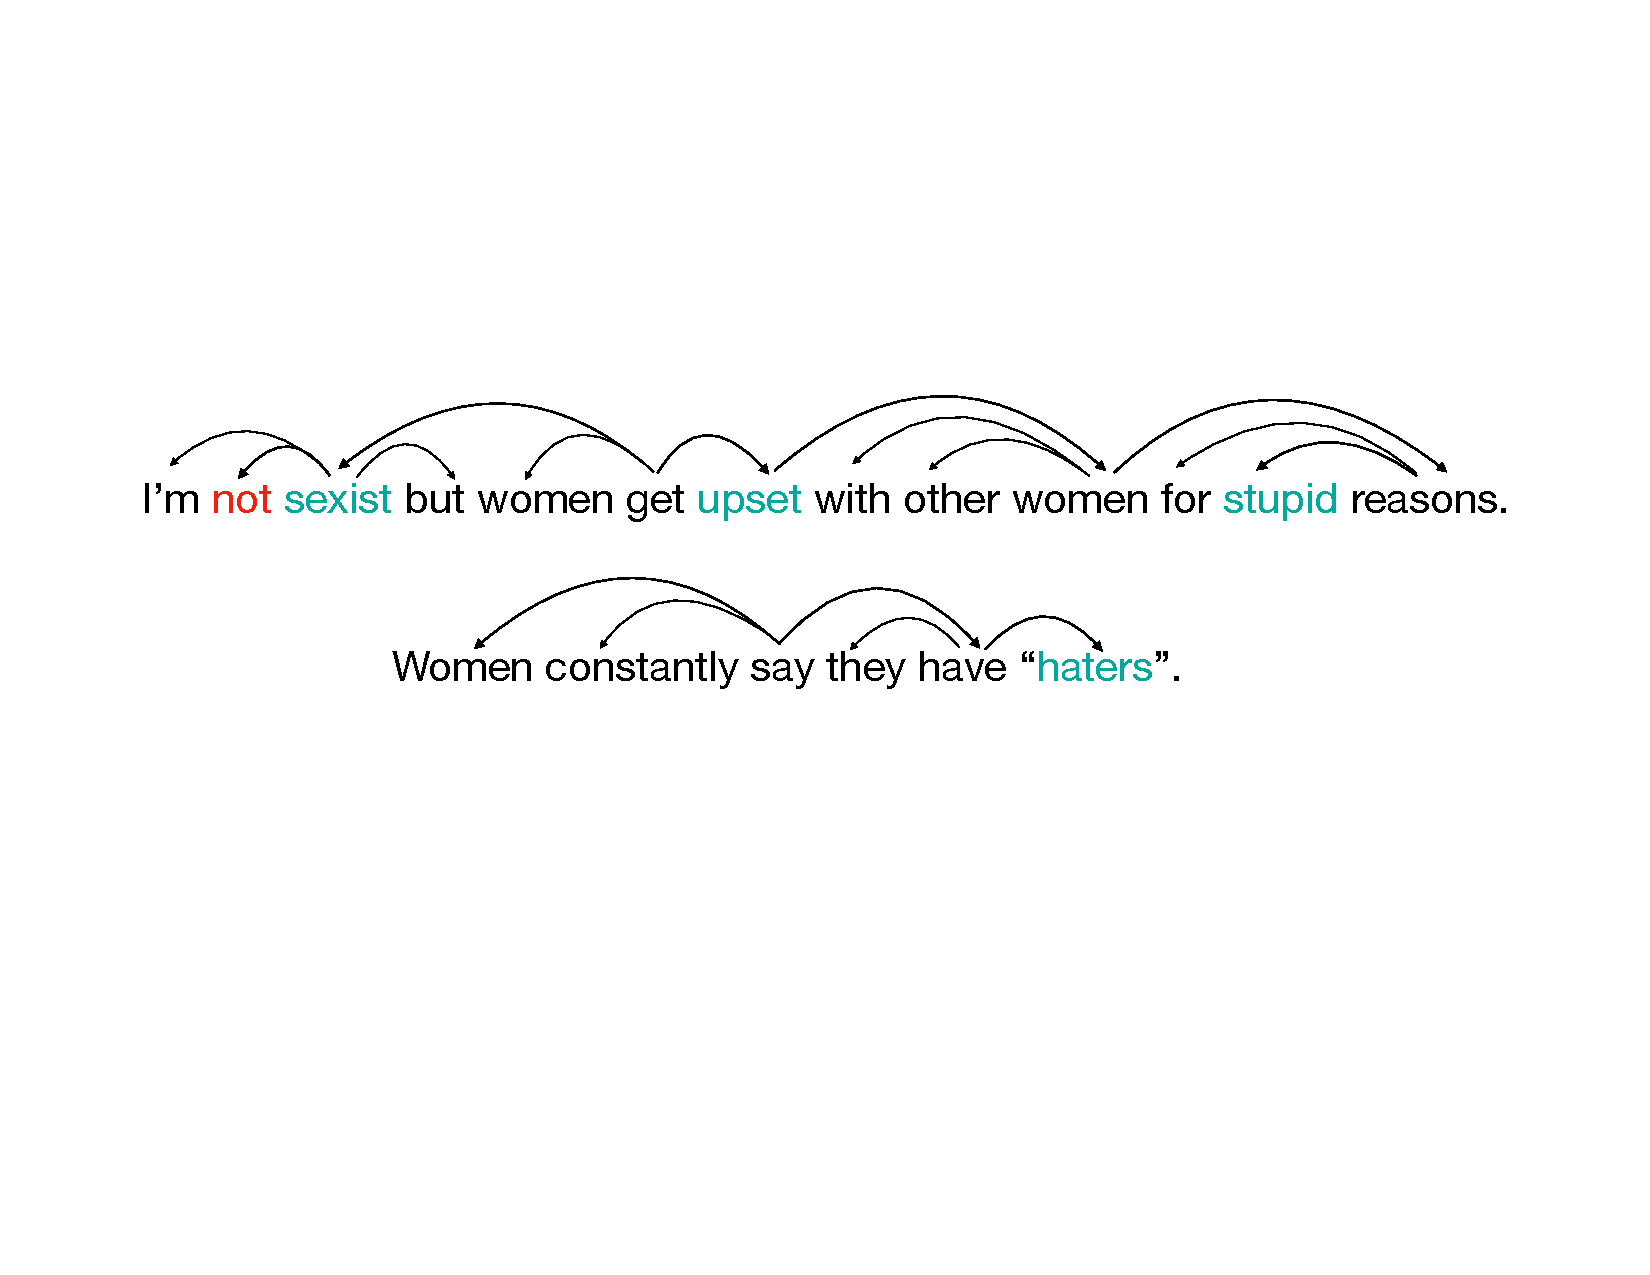
\includegraphics[scale=0.65]{figures/Example1_key}
  \caption{Parse tree of the sexist tweet missed by LSTM.}
  \label{fig:sample}
  \end{subfigure}

  \begin{subfigure}{\textwidth}
    \centering
    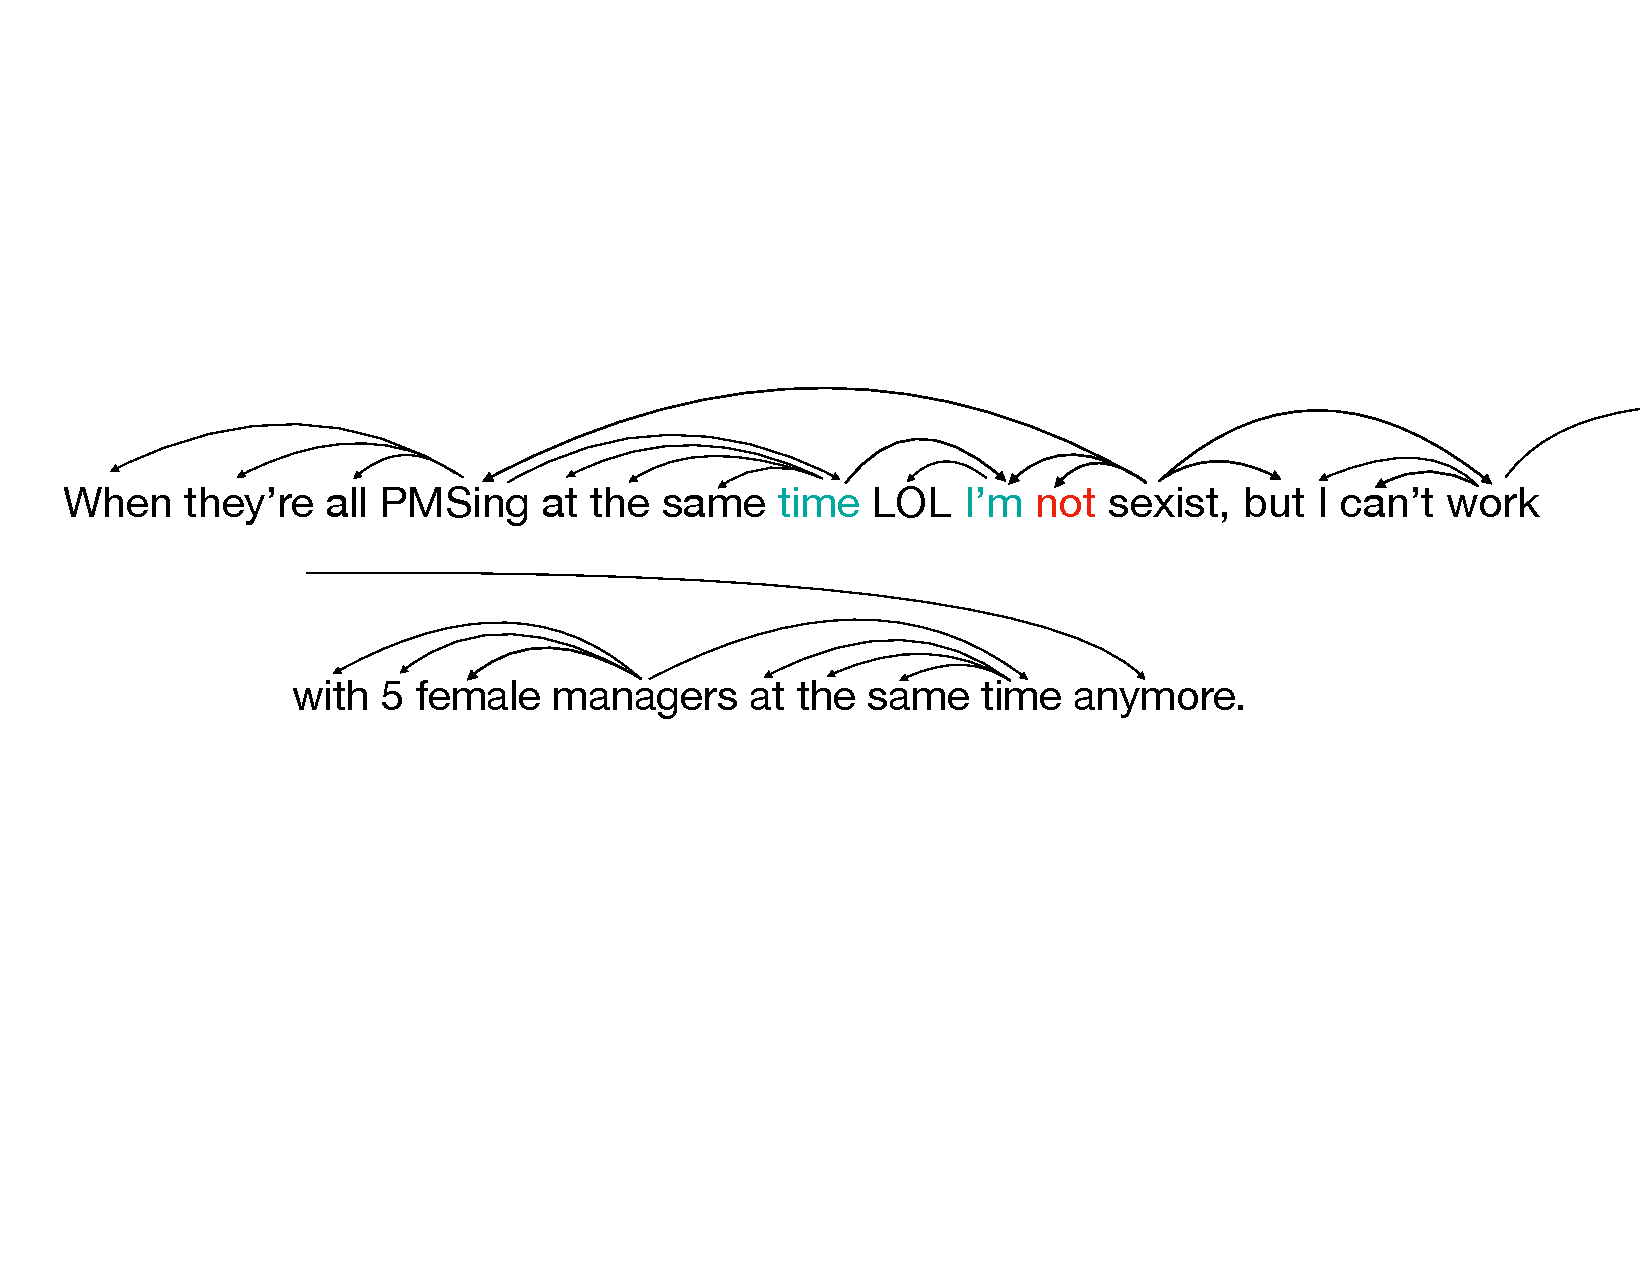
\includegraphics[scale=0.6]{figures/example2_key}
    \caption{Parse tree of the sexist tweet missed by DepGCN}
    \label{fig:example}
  \end{subfigure}

  \begin{subfigure}{\textwidth}
  \centering
    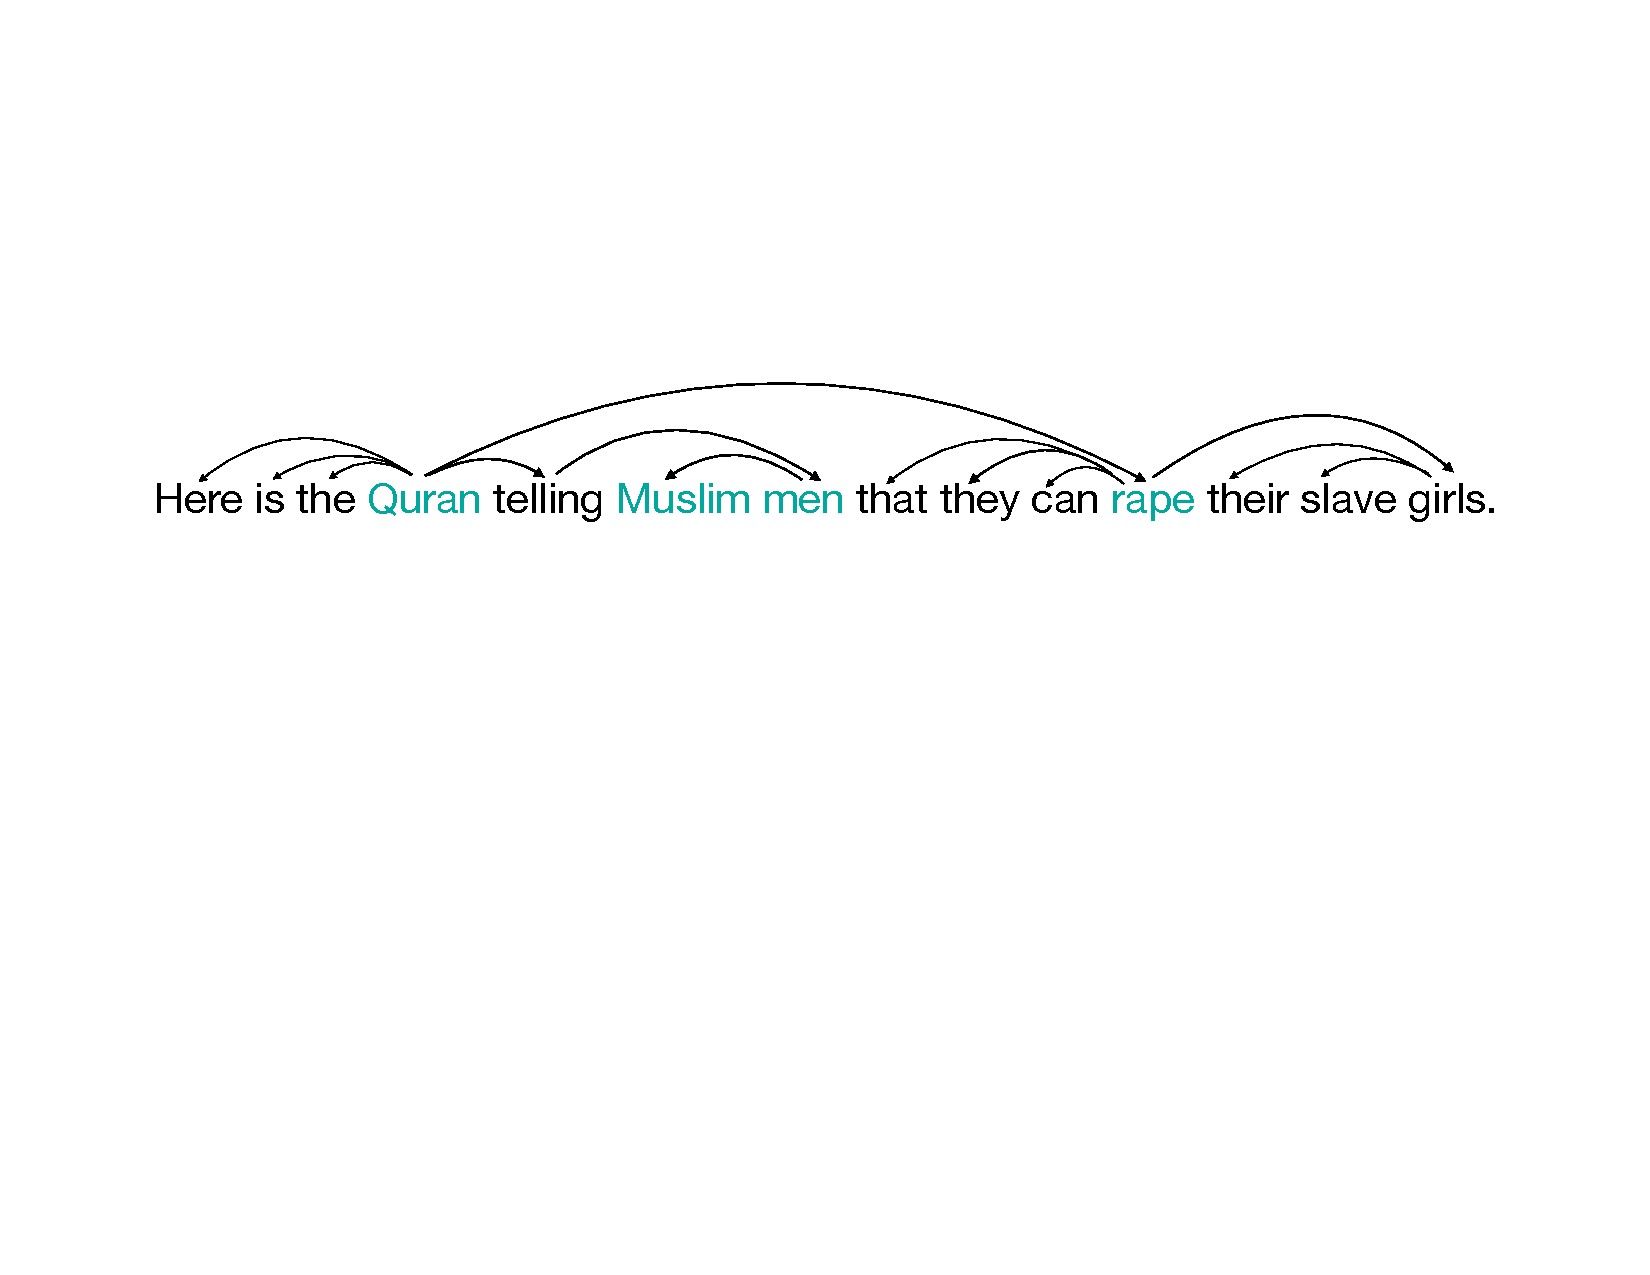
\includegraphics[scale=0.65]{figures/example3_key}
    \label{fig:example3}\caption{Parse tree of the racist tweet missed by DepGCN.}
    \end{subfigure}
    \begin{subfigure}{\textwidth}
    \centering
      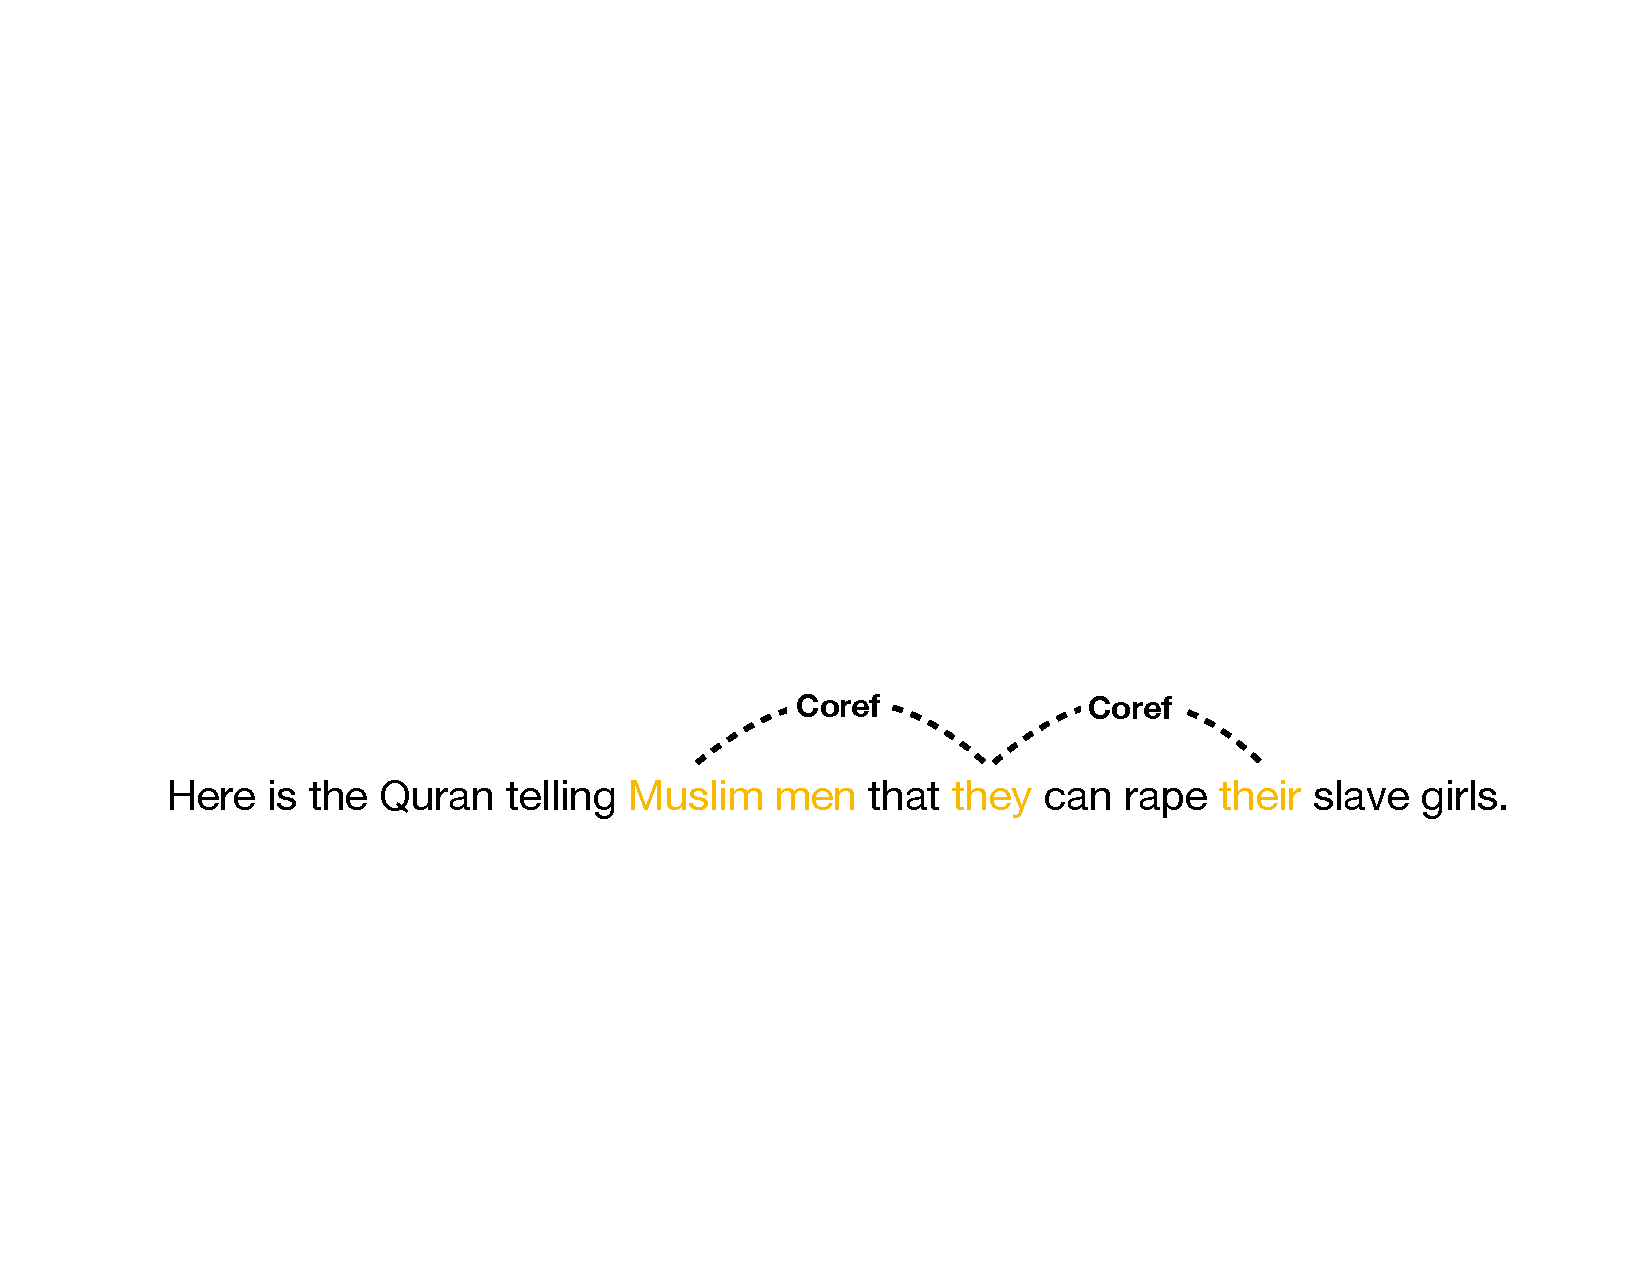
\includegraphics[scale=0.65]{figures/example3_2_key}
      \label{fig:examplecoref}\caption{Coreference resolution of the tweet.}
      \end{subfigure}

  \label{fig:examples}
  \caption{Parse Tree of the two sample tweets from Waseem dataset.}
\end{figure*}

\emph{Sexist tweet missed by LSTM}: Following is a sample sexist tweet that is correctly classified by the DepGCN approach but missed by the BiLSTM.
\textit{"I'm not sexist but women get upset with other women for stupid reasons. Women constantly say they have "haters"."}
\Cref{fig:sample} shows the parse tree of the tweet by the Stanford parser. It is a difficult sample to classify as the author of the tweet says that he is \textit{not} sexist but is writing offensive remarks against women. The dependency tree can capture this long-range dependency and establish negative relation of "upset," "stupid," and "haters" with the "women" subject.


\emph{Sexist tweet missed by DepGCN}: However, DepGCN fails to capture similar nuanced sexism in another sample tweet, \textit{"And when they're all PMSing at the same time LOL I'm not sexist, but I can't work with 5 female managers at the same time anymore.""}. Note that the sentence contains punctuation error as it is missing punctuation between the two sentences in the tweet (after \textit{time} and before \textit{I'm not}). This error leads to a wrong parse tree, as shown in \Cref{fig:example}. Thus, our parser-based model is sensitive to these parsing errors.

\emph{Racist tweet missed by DepGCN}: However, even if the parse tree is correct, just establishing dependency relationships may not be sufficient to capture nuanced relationships in the text. For instance, the parse tree of the racist tweet,
\textit{"Here is the Quran telling Muslim men that they can rape their slave girls."} shown in \Cref{fig:example3} is correct. However, the parse tree misses the coreference of pronouns \textit{they} and \textit{their} to belong to \textit{Muslim men}. In these cases, powerful language models like BERT will be able to extract these relationships.

\subsection{Effect of User Social Graph}
\Cref{tab:waseemuser} shows the class-wise F1 scores after adding the user social graph with the DepGCN model on the \citet{waseem-hovy-2016} dataset. We do not report results on the other datasets as we have do not have any information about their users. UserGCN used in isolation performs worse than the other approaches.
This poor performance is expected as it ignores the textual information entirely. Note that the UserGCN uses the user's class prior only for prediction for all of the user's tweets. However, even with that naive methodology, this model achieves similar performance to the previous state-of-the-art linguistic approach, N-gram (\Cref{tab:waseem}), and our DepGCN model for the sexist class.

\begin{table}[tbh]
  \centering
  \small
  \setlength{\tabcolsep}{2pt}
\begin{tabular}{ p{35mm} | c c  c c}
\toprule
 Approach &  Racist & Sexist & Clean & Overall \\
  \midrule
 BERT & 0.78 & 0.81 & 0.91 & 0.88 \\
 BiLSTM + DepGCN & \textbf{0.78} & 0.74 & 0.90 & 0.85 \\
 UserGCN & 0.61 & 0.72 & 0.79 & 0.74 \\
 BiLSTM+DepGCN \\ +UserGCN & \textbf{0.79} & \textbf{0.82} & \textbf{0.92} & \textbf{0.88} \\

 \bottomrule
\end{tabular}
\caption{\label{tab:waseemuser} Comparison of class-wise F1 score with weighted F1 score for different approaches with our proposed approach after adding the user social features on \citet{waseem-hovy-2016} dataset.}
\end{table}

After adding the user features, our model improves by 0.03 F1 points and slightly outperforms the previously best performing BERT model. The most significant improvement comes from the tweets annotated as sexist (similar trend seen in UserGCN). This improvement indicates that there is a strong homophily effect in users authoring sexist tweets in the dataset. As noted by \citet{mishra2019abusive}, racist tweets in this dataset are contributed by only five users who also tweet other benign and sexist tweets. Thus, incorporating additional user information does not give us higher gains for the racist class.
